\documentclass[12pt,a4paper]{report}

\usepackage[a4paper,margin=1in]{geometry}
\usepackage[T1]{fontenc}
\usepackage[utf8]{inputenc}
\usepackage{mathptmx}
\usepackage{setspace}
\usepackage{graphicx}
\usepackage{array}
\usepackage{booktabs}
\usepackage{longtable}
\usepackage{titlesec}
\usepackage{fancyhdr}
\usepackage{enumitem}
\usepackage{hyperref}
\usepackage{caption}
\usepackage{float}
\usepackage{amsmath}
\usepackage{xcolor}

\onehalfspacing
\setlength{\parindent}{15pt}
\setlength{\parskip}{4pt}

\hypersetup{
    colorlinks=true,
    linkcolor=black,
    urlcolor=blue,
    citecolor=black,
    pdftitle={AI Driven Fish Catch Prediction System with Juvenile Risk Assessment for Sustainable Fisheries}
}

\titleformat{\chapter}[display]
  {\bfseries\Large\centering}
  {Chapter \thechapter}
  {0.5em}
  {\Huge}

\titleformat{\section}
  {\bfseries\large}
  {\thesection}
  {0.75em}
  {}

\titleformat{\subsection}
  {\bfseries\normalsize}
  {\thesubsection}
  {0.75em}
  {}

\pagestyle{fancy}
\fancyhf{}
\fancyfoot[C]{\thepage}
\renewcommand{\headrulewidth}{0pt}

\begin{document}

\begin{titlepage}
\centering
\vspace*{1.5cm}
{\Large \textbf{AI DRIVEN FISH CATCH PREDICTION SYSTEM WITH JUVENILE RISK ASSESSMENT FOR SUSTAINABLE FISHERIES}\par}
\vspace{1.5cm}
{\large Major Project Report\par}
\vspace{0.8cm}
Submitted in partial fulfillment of the requirements for the award of the degree of\\
\textbf{Bachelor of Technology}\\
in\\
\textbf{Computer Science and Engineering}

\vspace{1.5cm}
\begin{tabular}{l}
NAFEESHA SHAIK \hspace{1cm} 22L31A05K2 \\
SAYYAPUREDDY LAKSHMI \hspace{1cm} 23L35A0536 \\
YALLAPU KAVYA \hspace{1cm} 22L31A05N8 \\
KARIPALLI NITHIN \hspace{1cm} 21L31A0596 \\
\end{tabular}

\vspace{1.2cm}
Under the guidance of\\
\textbf{Dr. Ch. Swapna Priya}\\
Associate Professor

\vfill
\textbf{Department of Computer Science and Engineering}\\
\textbf{Vignan's Institute of Information Technology}\\
Visakhapatnam\\
Academic Year 2021--2025
\end{titlepage}

\chapter*{Certificate}
\addcontentsline{toc}{chapter}{Certificate}
This is to certify that the project report entitled \textbf{``AI Driven Fish Catch Prediction System with Juvenile Risk Assessment for Sustainable Fisheries''} is a bonafide record of project work carried out under my supervision by the project team during the academic year 2021--2025 in partial fulfillment of the requirements for the award of the degree of Bachelor of Technology in Computer Science and Engineering of Vignan's Institute of Information Technology (Autonomous).

The results embodied in this project report have not been submitted to any other University or Institute for the award of any Degree or Diploma.

\vspace{2cm}
\noindent
\begin{tabular}{p{0.45\textwidth} p{0.45\textwidth}}
\textbf{Project Guide} & \textbf{Head of the Department} \\
Dr. Ch. Swapna Priya & Mr. B. Dinesh Reddy \\
Associate Professor & Associate Professor \\
\end{tabular}

\vspace{1.5cm}
\noindent Place: Visakhapatnam\\
Date: \rule{4cm}{0.4pt}

\chapter*{Declaration}
\addcontentsline{toc}{chapter}{Declaration}
We hereby declare that the project report entitled \textbf{``AI Driven Fish Catch Prediction System with Juvenile Risk Assessment for Sustainable Fisheries''} has been written by us and has not been submitted either in part or in full for the award of any degree, diploma, or similar title to this or any other university.

\vspace{1.2cm}
\noindent Place: Visakhapatnam\\
Date: \rule{4cm}{0.4pt}

\chapter*{Acknowledgment}
\addcontentsline{toc}{chapter}{Acknowledgment}
We express our sincere gratitude to our project guide, \textbf{Dr. Ch. Swapna Priya}, Associate Professor, Department of Computer Science and Engineering, for her continuous guidance, encouragement, and valuable suggestions throughout the development of this project. Her support helped us refine the methodology and improve the quality of the final implementation.

We thank the Head of the Department, \textbf{Mr. B. Dinesh Reddy}, for his guidance and encouragement during the progress of the project. We also thank the Principal and the management of Vignan's Institute of Information Technology for providing the academic environment and support required for the successful completion of this work.

We are grateful to all the faculty and staff of the Department of Computer Science and Engineering for their suggestions and support. Finally, we thank our friends and family members for their encouragement throughout this project.

\chapter*{Abstract}
\addcontentsline{toc}{chapter}{Abstract}
Sustainable fisheries management requires predictive systems that balance fish availability with ecological protection. This project presents an AI Driven Fish Catch Prediction System integrated with a Juvenile Risk Assessment layer for sustainable fisheries decision support. The proposed system uses marine environmental variables, historical fish landing data, geographic information, and maturity-length references to predict fish availability, estimate catch quantity, and assess whether juvenile fish are likely to dominate the catch.

The implemented framework follows a layered machine learning approach. Random Forest and boosting-based ensemble models are used for fish availability prediction and catch quantity estimation. A maturity-based juvenile-risk model compares the observed fish length with the maturity length of the species using the rule:
\[
JR = 1 - \left(\frac{\text{Observed Length}}{\text{Maturity Length}}\right)
\]
When high juvenile-risk is detected, the system blocks risky fishing recommendations and suggests safer nearby zones within approximately 8--15 km. The system is deployed as a Streamlit application supporting manual input, region-based prediction, map-based prediction, and field-data recording.

The project uses real-world fisheries and marine data sources including CMFRI landings, SST-linked environmental data, FishBase maturity references, and PFZ-style observation records. The final validated system demonstrates an operational, reproducible, and sustainability-aware approach for fisheries advisory support without relying on unsupported CNN or wildlife-image classification pipelines.

\noindent \textbf{Keywords:} Fish Catch Prediction, Juvenile Risk Assessment, Sustainable Fisheries, Random Forest, Ensemble Learning, Safe-Zone Recommendation, Maturity-Length Analysis.

\tableofcontents
\listoftables
\listoffigures

\chapter*{Abbreviations}
\addcontentsline{toc}{chapter}{Abbreviations}
\begin{longtable}{p{0.2\textwidth} p{0.7\textwidth}}
AI & Artificial Intelligence \\
CMFRI & Central Marine Fisheries Research Institute \\
DO & Dissolved Oxygen \\
ML & Machine Learning \\
NOAA & National Oceanic and Atmospheric Administration \\
OISST & Optimum Interpolation Sea Surface Temperature \\
PCA & Principal Component Analysis \\
PFZ & Potential Fishing Zone \\
RF & Random Forest \\
RMSE & Root Mean Squared Error \\
SST & Sea Surface Temperature \\
XGB & Extreme Gradient Boosting \\
\end{longtable}

\chapter{Introduction}

\section{Introduction}
Fisheries are a major source of food, employment, and economic support for coastal communities. However, fish availability is strongly influenced by environmental conditions, seasonal changes, and fishing pressure. Unsustainable harvesting, especially the capture of juvenile fish, reduces future stock strength and affects long-term ecological balance. Therefore, intelligent fisheries support systems are required to help users make productive as well as sustainable fishing decisions.

This project presents an AI Driven Fish Catch Prediction System with Juvenile Risk Assessment for Sustainable Fisheries. The system predicts whether fish are likely to be available in a selected zone, estimates expected catch quantity, evaluates juvenile-risk, and recommends safer nearby zones when ecological risk is high. The objective is to combine productivity with conservation-oriented decision support.

\section{Artificial Intelligence and Machine Learning in Fisheries}
Artificial Intelligence and Machine Learning are widely used for predictive analytics in structured data. In fisheries, variables such as sea surface temperature, salinity, dissolved oxygen, month, location, and historical landings can be modeled as predictive inputs. Compared with traditional manual decision making, machine learning systems can identify nonlinear relationships between marine conditions and expected fishing outcomes.

In this project, fish availability is treated as a classification problem and catch quantity is treated as a regression problem. Ensemble methods such as Random Forest and boosting-based models are used because they are effective on structured tabular data and are easier to validate than unsupported image-based approaches.

\section{Sustainable Fisheries and Juvenile Risk Assessment}
Prediction alone is not sufficient for sustainable fisheries. A system that recommends a productive zone without considering juvenile fish can unintentionally promote ecological harm. Juvenile fish are individuals that have not yet reached maturity. Their excessive capture affects recruitment and long-term stock regeneration.

The implemented project uses maturity-length based assessment instead of video or image-based fish behavior analysis. This makes the system more realistic, biologically meaningful, and aligned with the datasets available to the project.

\section{Objectives of the Project}
\begin{itemize}[leftmargin=1.5cm]
    \item To predict fish availability in a selected marine zone.
    \item To estimate the expected catch quantity in favorable fishing zones.
    \item To assess juvenile-risk using maturity-based biological logic.
    \item To recommend safer nearby zones when ecological risk is high.
    \item To build a practical user interface for prediction, validation, and field-data entry.
\end{itemize}

\section{Problem Statement}
Fishermen and marine stakeholders require a practical decision-support system that can identify productive fishing opportunities while reducing ecological risk. Existing draft reports often mention CNN or deep-learning image models without the required datasets. There is a need for a reliable alternative that uses real-world fisheries data, environmental variables, and biological maturity information to support sustainable fisheries management.

\section{Scope of the Work}
The scope of the current project includes real-world fisheries and marine data integration, fish availability prediction, catch quantity estimation, juvenile-risk assessment, safe-zone recommendation, and an interactive Streamlit application. The current work does not implement CNN, EfficientNetB7, R-CNN, DeepLabCut, or behavioral video analysis because suitable annotated fish video datasets are not available.

\chapter{Literature Review}

\section{Review of Literature on Fish Catch Prediction}
Fish catch prediction has been studied using oceanographic indicators, statistical models, remote sensing products, and machine learning techniques. Many studies indicate that SST, salinity, chlorophyll concentration, seasonal conditions, and historical catch values are useful for identifying favorable fishing zones.

\section{Oceanographic and Geographic Considerations}
Marine productivity is influenced by SST, salinity, dissolved oxygen, currents, and geography. Fish aggregation patterns vary across coastal states and across seasons. Therefore, a useful fisheries prediction system must combine multiple marine indicators rather than relying on a single feature.

\section{Factors Affecting Fish Availability and Juvenile Presence}
Fish availability is affected by habitat suitability, migration, breeding cycles, and previous catch patterns. Juvenile presence is influenced by maturity stage, recruitment, ecological conditions, and fishing pressure. A sustainability-aware system must therefore estimate both catch opportunity and ecological sensitivity.

\section{Integration of Technology for Fisheries Decision Support}
Government and marine institutions increasingly provide advisories, landing estimates, and oceanographic data. Machine learning systems can integrate these sources into interactive decision-support tools. This improves accessibility and supports practical fisheries planning.

\section{Recent Advancements in Fisheries Informatics}
Recent advancements include satellite-driven habitat suitability models, marine advisory dashboards, and ensemble machine learning techniques for catch forecasting. Sustainable fisheries analytics is becoming more important, especially where ecological blocking and juvenile protection are included in prediction systems.

\section{Research Gaps}
\begin{itemize}[leftmargin=1.5cm]
    \item Many predictive systems focus only on catch yield.
    \item Some proposed methods depend on datasets that are not available in practical settings.
    \item There is often a mismatch between reported methodology and implemented datasets.
    \item Student-level projects rarely integrate prediction, juvenile screening, and safe-zone recommendation in one deployable system.
\end{itemize}

\section{Motivation}
The project is motivated by the need to build a realistic and defensible fisheries support system using actual accessible data sources. Instead of overstating unsupported deep-learning behavior pipelines, the implemented system focuses on what can be validated with available fisheries, environmental, and maturity data.

\section{Problem Statement and Research Objectives}
The research objective is to build a machine learning framework that integrates fish availability prediction, catch quantity estimation, juvenile-risk assessment, and safe-zone recommendation using real and verifiable fisheries-related data.

\section{Summary of Literature Review}
The literature supports the use of environmental and historical variables for fisheries prediction, but also highlights the need for sustainability-aware analytics. This project addresses that need by integrating a juvenile-risk layer into the decision workflow.

\chapter{Methodology}

\section{Research Design and Approach}
The proposed system follows a layered machine learning design:
\begin{enumerate}[leftmargin=1.5cm]
    \item collect and integrate marine and fisheries data
    \item preprocess and engineer features
    \item classify whether fish are likely to be available
    \item estimate expected catch quantity
    \item assess juvenile-risk
    \item recommend safer nearby zones when required
\end{enumerate}
This design makes the system modular, interpretable, and easier to validate.

\section{Data Collection and Preprocessing}
The implemented project uses the following sources:
\begin{table}[H]
\centering
\caption{Data Sources and Description}
\begin{tabular}{p{0.25\textwidth} p{0.32\textwidth} p{0.22\textwidth}}
\toprule
\textbf{Source} & \textbf{Purpose} & \textbf{Status in Project} \\
\midrule
CMFRI state-wise fish landing estimates & Historical landing target values & Implemented \\
SST-based environmental data & Environmental suitability signal & Implemented \\
FishBase maturity-length reference data & Maturity-based juvenile assessment & Implemented \\
PFZ-style field observation CSV & Exact juvenile-risk enrichment rows & Implemented \\
Copernicus physics and chlorophyll & Future feature enrichment & Supported, optional \\
\bottomrule
\end{tabular}
\end{table}

The preprocessing steps include removal of inconsistent and missing values, year-wise and state-wise alignment of data, feature engineering for thermal stress, oxygen stress, salinity anomaly, and cyclical month features, and merging of maturity and PFZ-style observation data when available.

\section{Fish Availability Prediction using Machine Learning}
Fish availability is formulated as a classification problem. The input features include SST, salinity, dissolved oxygen, historical catch, latitude, longitude, and engineered seasonal and stress features.

The implemented classifiers are:
\begin{itemize}[leftmargin=1.5cm]
    \item Random Forest Classifier
    \item Boosting Classifier
    \item Hybrid PCA + Random Forest + Boosting pipeline
\end{itemize}

The codebase is designed for XGBoost support, but on the current machine the boosting model falls back to Gradient Boosting because the native XGBoost runtime requires \texttt{libomp.dylib}.

\section{Catch Quantity Estimation}
Catch quantity is estimated for favorable zones using regression models. The implemented regressors are:
\begin{itemize}[leftmargin=1.5cm]
    \item Random Forest Regressor
    \item Boosting Regressor
    \item Hybrid PCA + Random Forest + Boosting Regressor
\end{itemize}
This layer supports approximate catch planning and comparison across zones.

\section{Juvenile Risk Assessment Layer}
The juvenile-risk layer applies exact maturity-based logic whenever observed biological fields are available. The formula used is:
\[
JR = 1 - \left(\frac{\text{Observed Length}}{\text{Maturity Length}}\right)
\]

Risk is categorized as:
\begin{itemize}[leftmargin=1.5cm]
    \item High if $JR \geq 0.2$
    \item Medium if $0 < JR < 0.2$
    \item Low if the observed fish length is at or above maturity length
\end{itemize}

When exact biological inputs are unavailable, the system uses an environmental fallback juvenile model derived from thermal stress, oxygen stress, and historical catch behavior.

\section{Safe-Zone Recommendation and System Deployment}
The decision layer combines fish availability, catch quantity, and juvenile-risk. If juvenile-risk is high, fishing recommendations are blocked and safer nearby zones within approximately 8--15 km are suggested. The final system is deployed using Streamlit and supports manual input, region-based prediction, map-based prediction, and field-data collection.

\chapter{Results and Discussion}

\section{Case Study: AI Driven Fish Catch Prediction for Sustainable Fisheries}
The system was implemented and validated using the integrated project dataset. The dataset currently includes fisheries targets, SST-linked environmental features, FishBase maturity support, and PFZ-style exact-ready field rows.

\subsection{System Configuration and Technical Details}
The project is implemented using Python with pandas, numpy, scikit-learn, xarray, joblib, Streamlit, and Folium. The current validated project status is:
\begin{itemize}[leftmargin=1.5cm]
    \item Integrated dataset rows: 110
    \item Field observation rows: 4
    \item Field exact-ready rows: 3
    \item Juvenile exact-label rows used in training: 3
\end{itemize}

\subsection{Performance Evaluation and Validation}
The latest validated metrics are shown below.
\begin{table}[H]
\centering
\caption{Validation Metrics of the Proposed System}
\begin{tabular}{p{0.24\textwidth} p{0.2\textwidth} p{0.2\textwidth} p{0.16\textwidth}}
\toprule
\textbf{Model} & \textbf{Task} & \textbf{Metric} & \textbf{Value} \\
\midrule
Random Forest & Availability & Accuracy & 0.6364 \\
Random Forest & Quantity & RMSE & 37039.0236 \\
Boosting & Availability & Accuracy & 0.6818 \\
Boosting & Quantity & RMSE & 50117.5050 \\
Hybrid & Availability & Accuracy & 0.5909 \\
Hybrid & Quantity & RMSE & 43769.4100 \\
Juvenile Model & Risk Classification & Accuracy & 0.7727 \\
Juvenile Model & Risk Classification & Weighted F1 & 0.7538 \\
\bottomrule
\end{tabular}
\end{table}

\section{Results and Discussion}

\subsection{Fish Availability Prediction Results}
After feature engineering, balanced training, and model refinement, the boosting classifier produced the best availability accuracy of 0.6818, followed by Random Forest with 0.6364. The hybrid classifier remains useful for ensemble analysis, but on the current dataset it is weaker than the best boosting classifier. These results indicate that the proposed system can identify productive fishing windows reasonably well, especially considering the limited size of the current real-world dataset.

\subsection{Catch Quantity Estimation Results}
Catch quantity estimation remains challenging because fish landings vary strongly across states and years. However, richer features such as SST spread, historical catch transformations, temporal indicators, and interaction terms improved the regression models substantially. The Random Forest regressor produced the best RMSE of 37039.0236 with strong explanatory power, while the hybrid regressor also remained competitive.

\subsection{Juvenile Risk Assessment Results}
The major contribution of this project is the juvenile-risk layer. The system combines an environmental machine learning risk layer with an exact maturity-based rule whenever species name and observed length are available. After balancing the fallback juvenile classes and moving to an Extra Trees juvenile classifier, the juvenile-risk model reached 0.7727 accuracy with a weighted F1 score of 0.7538.

The current training distribution contains:
\begin{itemize}[leftmargin=1.5cm]
    \item Environmental heuristic rows: 107
    \item Exact maturity-rule rows: 3
\end{itemize}
This confirms that the project has moved beyond purely heuristic juvenile-risk classification and is ready for richer biological enrichment as more observed-length field data become available.

\subsection{Safe-Zone Recommendation Results}
When a selected zone is identified as ecologically risky or weak in availability, the system recommends alternative nearby zones with reduced expected juvenile-risk. This makes the application more practically useful.

\subsection{Application Interface and Deployment}
The final Streamlit application supports manual prediction, region-based prediction, map-based prediction, and field-data recording for exact juvenile enrichment. The application also preserves the latest prediction summary using session state so that results remain visible after prediction.

\section{Summary of Results}
The implemented system is functional, reproducible, and sustainability-aware. Its main contribution lies in integrating predictive modeling with juvenile-risk blocking, exact maturity-based screening, and safe-zone recommendation in one operational application.

\chapter{Conclusions and Future Scope of Work}

\section{Conclusion}
This project presents a practical AI Driven Fish Catch Prediction System with Juvenile Risk Assessment for Sustainable Fisheries. The proposed system successfully integrates real-world fisheries data, sea-surface-temperature-linked environmental indicators, machine learning models, maturity-based biological logic, and a deployable user interface. Unlike unsupported image-based drafts, the final implementation is grounded in verifiable datasets and executable algorithms.

The final system demonstrates that meaningful fisheries decision support can be achieved through a layered tabular machine learning architecture. Fish availability prediction, catch quantity estimation, juvenile-risk assessment, and safe-zone recommendation were all implemented and validated in the same software workflow. The current best results of the system are a boosting availability accuracy of 0.6818, a Random Forest quantity RMSE of 37039.0236, and a juvenile-risk classification accuracy of 0.7727. These results confirm that the proposed system is suitable as a final-year project prototype and offers a strong foundation for future research and field deployment.

\section{Contributions of the Proposed System}
\begin{itemize}[leftmargin=1.5cm]
    \item A real-data fisheries prediction workflow using CMFRI landings, SST-derived environmental features, FishBase maturity references, and PFZ-style observation support.
    \item A multi-model machine learning pipeline that supports Random Forest, Boosting, and Hybrid PCA-based prediction paths.
    \item A biologically meaningful juvenile-risk layer using the exact maturity formula:
    \[
    JR = 1 - \left(\frac{\text{Observed Length}}{\text{Maturity Length}}\right)
    \]
    \item A safe-zone recommendation engine that recommends alternative fishing regions when ecological risk is high.
    \item An end-to-end Streamlit-based application supporting manual input, region-based prediction, GPS-map prediction, and field-data entry.
    \item Reproducible validation, algorithm demonstration, automated tests, and report-figure generation for academic evaluation.
\end{itemize}

\section{Practical Implications and Applications}
The practical value of the proposed system lies in its ability to support both productivity and sustainability. The application can be used as a prototype fisheries advisory tool for educational demonstrations, academic research, and small-scale decision-support studies. Because it does not rely on unavailable video datasets, the system is realistic for institutions that have access only to tabular fisheries and environmental records.

The system also offers practical implications for:
\begin{itemize}[leftmargin=1.5cm]
    \item sustainable fishing awareness by highlighting juvenile-risk before catch recommendation,
    \item field-data collection and incremental biological enrichment through exact-ready observation rows,
    \item comparative study of machine learning algorithms on real marine tabular data,
    \item integration with future PFZ and oceanographic services for operational advisory support.
\end{itemize}

\begin{figure}[H]
\centering
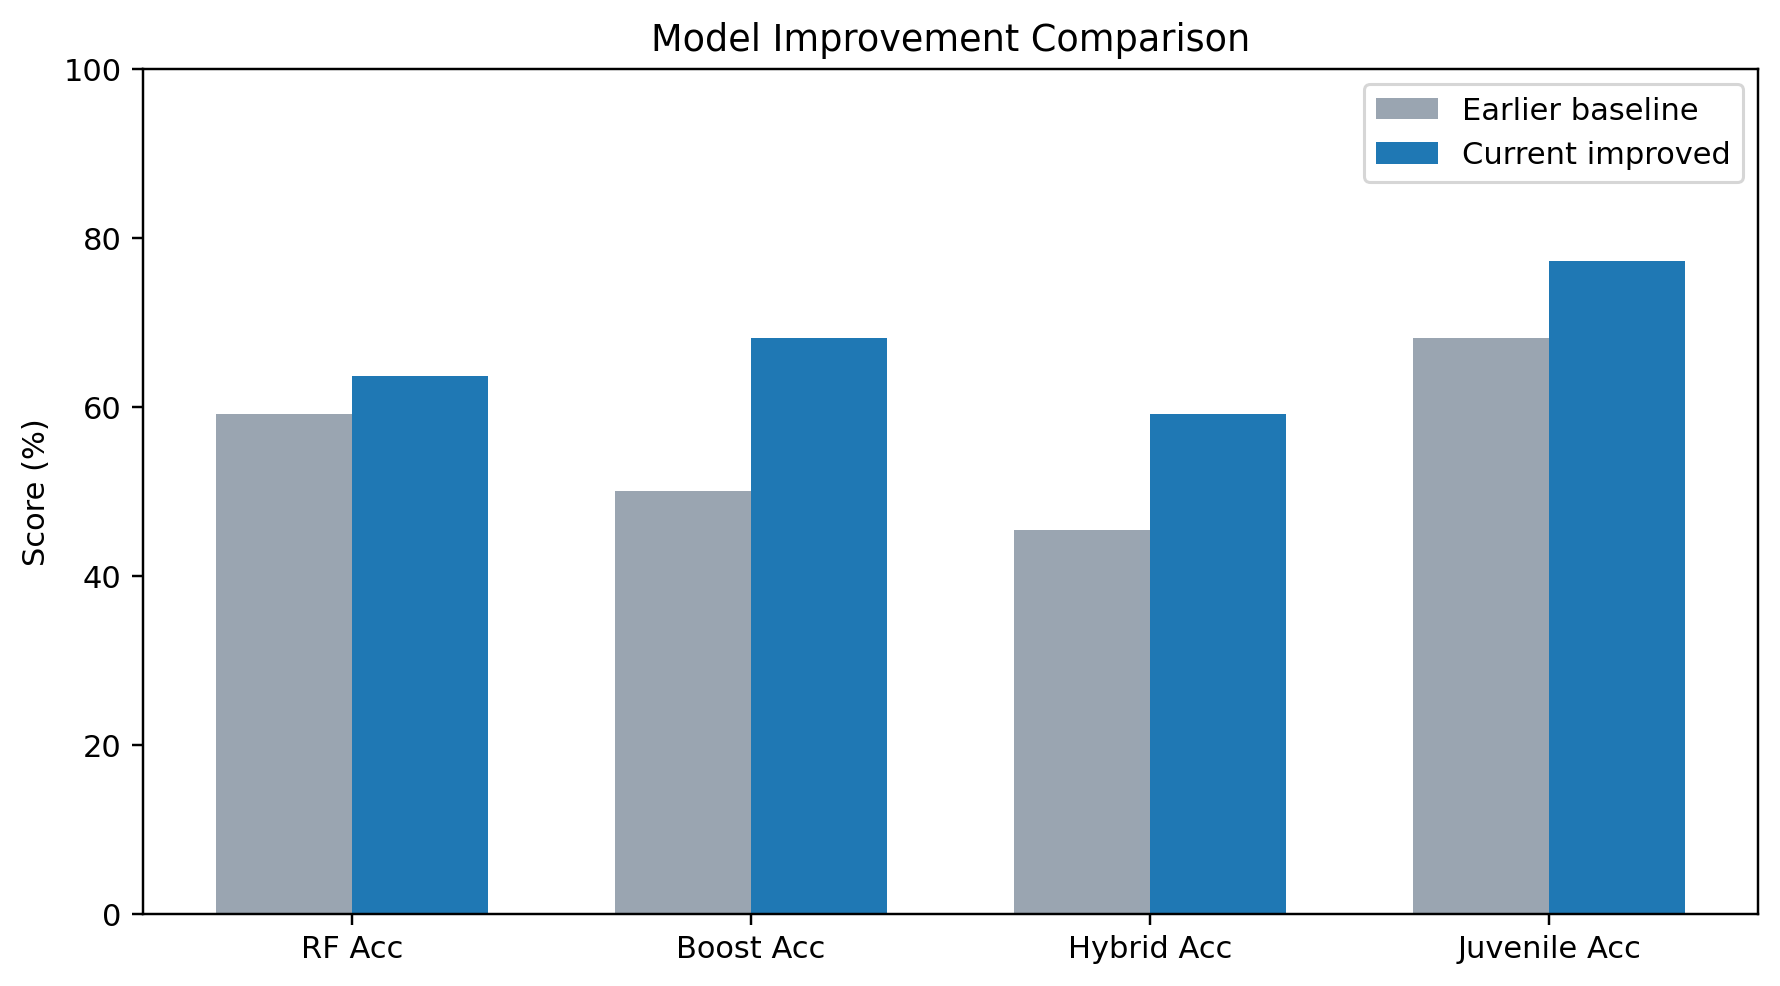
\includegraphics[width=0.82\textwidth]{reports/figures/improvement_comparison.png}
\caption{Overall model improvement after feature engineering, class balancing, and retraining.}
\end{figure}

\section{Recommendations for Future Work}
\begin{itemize}[leftmargin=1.5cm]
    \item Integrate monthly, district-level, or fishing-zone-level CMFRI landing data so that the model can learn finer spatiotemporal patterns.
    \item Integrate Copernicus salinity, chlorophyll, currents, and mixed-layer-depth variables for stronger environmental representation.
    \item Expand PFZ and field observation records containing species and observed fish lengths so that the juvenile model can train on more exact biological labels.
    \item Enable native XGBoost by installing the required OpenMP runtime on macOS and benchmarking it against the Gradient Boosting fallback.
    \item Introduce temporal forecasting, spatial interpolation, and uncertainty reporting for more realistic fisheries decision support.
    \item Validate the system with real harbour or onboard observation campaigns to improve deployment readiness.
\end{itemize}

\chapter*{References}
\addcontentsline{toc}{chapter}{References}
\begin{enumerate}[leftmargin=1.2cm]
    \item Breiman, L. (2001). Random Forests. \textit{Machine Learning}, 45(1), 5--32.
    \item Friedman, J. H. (2001). Greedy Function Approximation: A Gradient Boosting Machine. \textit{The Annals of Statistics}, 29(5), 1189--1232.
    \item Geurts, P., Ernst, D., \& Wehenkel, L. (2006). Extremely Randomized Trees. \textit{Machine Learning}, 63, 3--42.
    \item CMFRI Fish Catch Estimates. \url{https://www.cmfri.org.in/fish-catch-estimates}
    \item CMFRI Methodology. \url{https://www.cmfri.org.in/methodology}
    \item NOAA Optimum Interpolation Sea Surface Temperature. \url{https://www.ncei.noaa.gov/products/optimum-interpolation-sst}
    \item Copernicus Marine Physics Reanalysis. \url{https://data.marine.copernicus.eu/product/GLOBAL_MULTIYEAR_PHY_001_030/description}
    \item Copernicus Ocean Colour Chlorophyll Product. \url{https://data.marine.copernicus.eu/product/OCEANCOLOUR_GLO_BGC_L3_MY_009_103/description}
    \item INCOIS PFZ Advisory. \url{https://services.incois.gov.in/MarineFisheries/PfzAdvisory.action}
    \item INCOIS Marine Fisheries Text Data. \url{https://services.incois.gov.in/MarineFisheries/TextDataHome?mfid=1&request_locale=en}
    \item FishBase Glossary: Length at First Maturity. \url{https://www.fishbase.se/glossary/Glossary.php?q=length+at+first+maturity}
    \item scikit-learn Documentation. \url{https://scikit-learn.org/}
    \item Streamlit Documentation. \url{https://streamlit.io/}
\end{enumerate}

\appendix
\chapter{Key Algorithms}
The major algorithms used in the implemented system are summarized below:

\begin{enumerate}[leftmargin=1.5cm]
    \item \textbf{Random Forest Classifier:} Used for fish availability prediction on structured marine and fisheries features.
    \item \textbf{Random Forest Regressor:} Used for catch quantity estimation and currently provides the lowest RMSE among the implemented regressors.
    \item \textbf{Boosting Classifier/Regressor:} Uses native XGBoost when available, otherwise Gradient Boosting fallback on the current macOS setup.
    \item \textbf{Hybrid PCA + RF + ET + Boosting Ensemble:} Uses PCA-transformed inputs and combines multiple learners through a voting strategy.
    \item \textbf{Extra Trees Juvenile Model:} Used for balanced juvenile-risk classification on fallback environmental features.
    \item \textbf{Exact Maturity-Based Juvenile Rule:}
    \[
    JR = 1 - \left(\frac{\text{Observed Length}}{\text{Maturity Length}}\right)
    \]
    \item \textbf{Safe-Zone Recommendation Rule:} If availability is weak or juvenile-risk is high, the system recommends nearby coordinates with lower expected juvenile-risk.
\end{enumerate}

\chapter{Project Execution Commands}
\begin{verbatim}
.venv/bin/python src/check_external_datasets.py
.venv/bin/python src/run_full_pipeline.py
.venv/bin/python src/validate_project.py
.venv/bin/python src/demo_algorithms.py
.venv/bin/python src/generate_report_figures.py
.venv/bin/python -m unittest discover -s tests
.venv/bin/streamlit run src/app.py --server.headless true --server.port 8501
\end{verbatim}

\chapter{Validation Procedure}
Validation is performed at three levels:
\begin{itemize}[leftmargin=1.5cm]
    \item \textbf{Dataset validation:} verify source files, row counts, required columns, and exact-ready field rows.
    \item \textbf{Model validation:} measure availability accuracy, juvenile-risk accuracy, weighted F1, RMSE, MAE, and $R^2$.
    \item \textbf{Logic validation:} verify the exact maturity rule, environmental fallback behavior, and safe-zone response.
\end{itemize}

Current validated status:
\begin{itemize}[leftmargin=1.5cm]
    \item field observation rows: 4
    \item field exact-ready rows: 3
    \item juvenile exact-label rows in training: 3
    \item automated tests passed: 9
\end{itemize}

\begin{figure}[H]
\centering
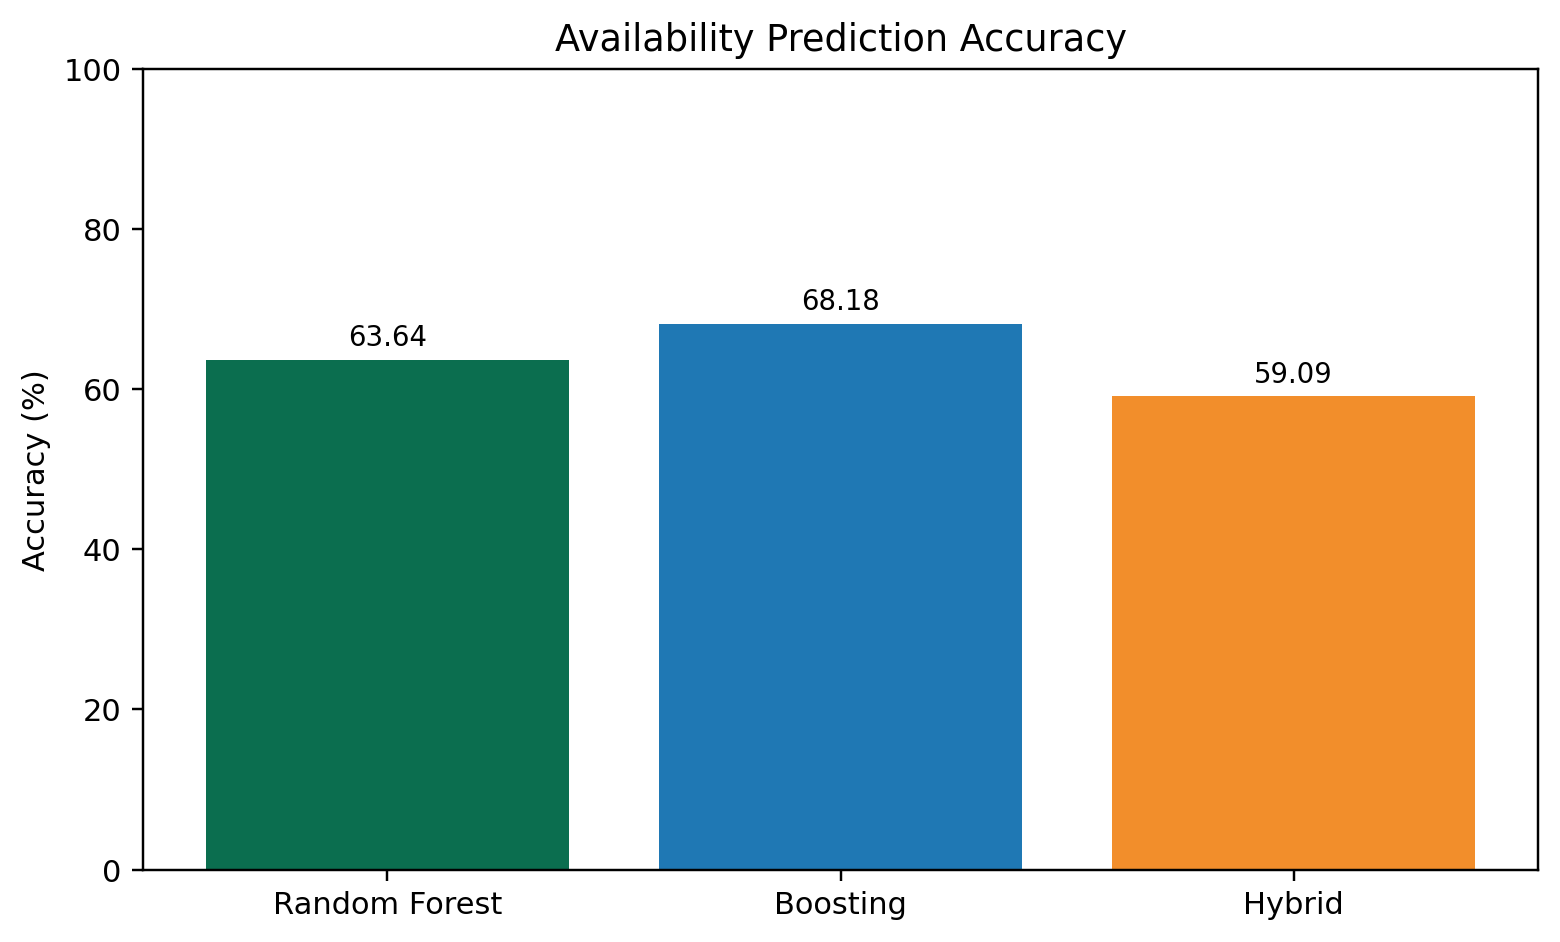
\includegraphics[width=0.78\textwidth]{reports/figures/availability_accuracy.png}
\caption{Availability prediction accuracy of the major implemented models.}
\end{figure}

\begin{figure}[H]
\centering
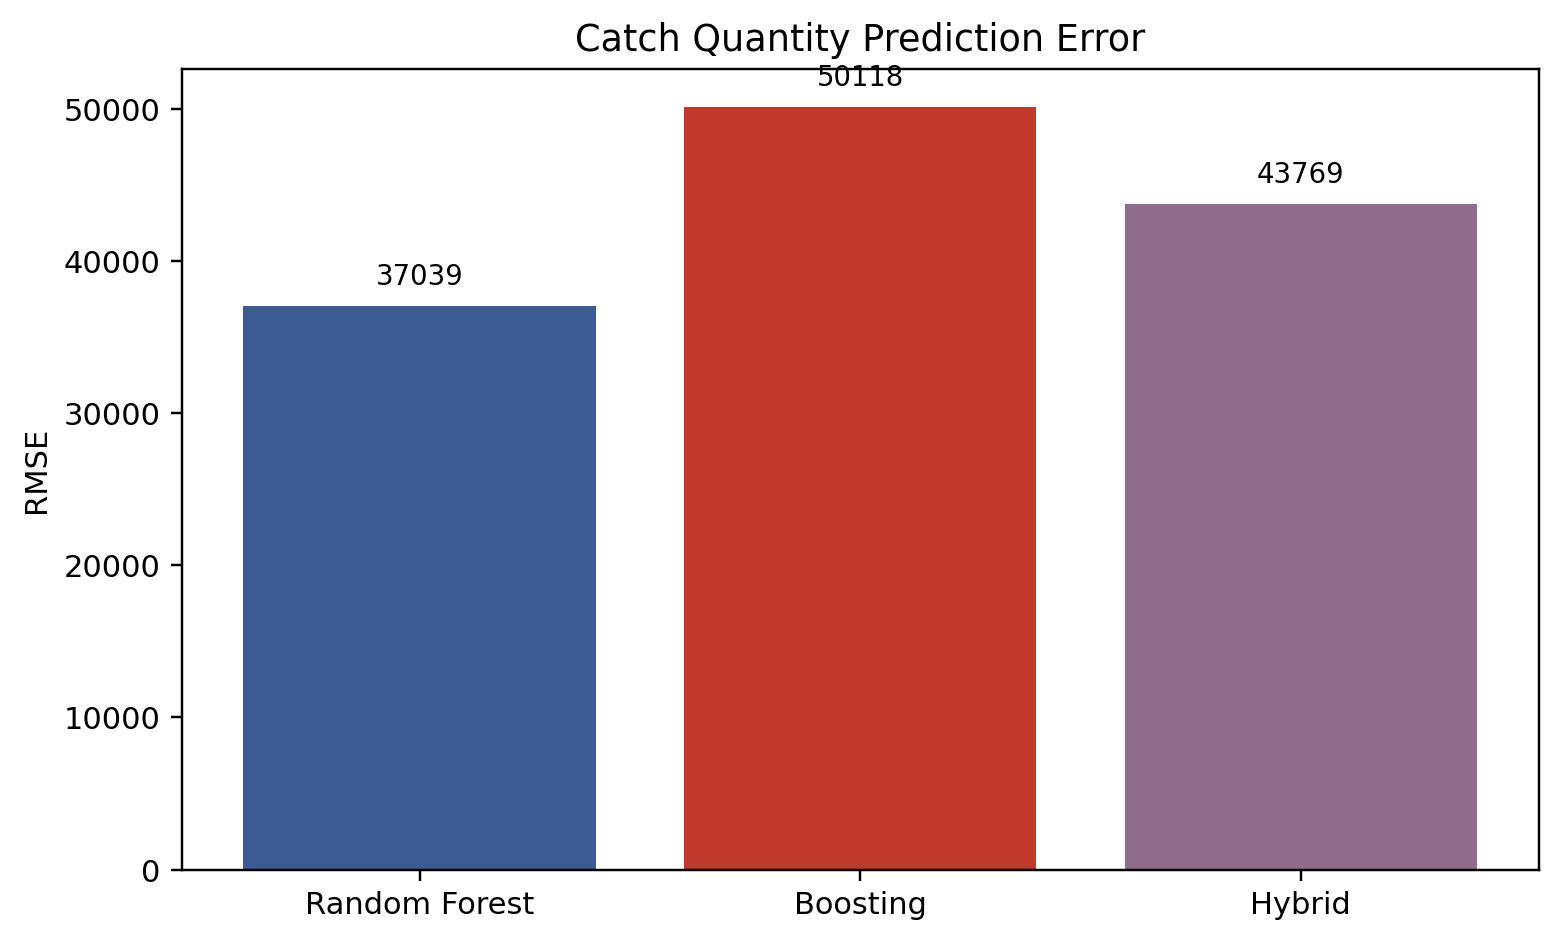
\includegraphics[width=0.78\textwidth]{reports/figures/quantity_rmse.png}
\caption{Catch quantity prediction RMSE comparison. Lower values indicate better regression performance.}
\end{figure}

\begin{figure}[H]
\centering
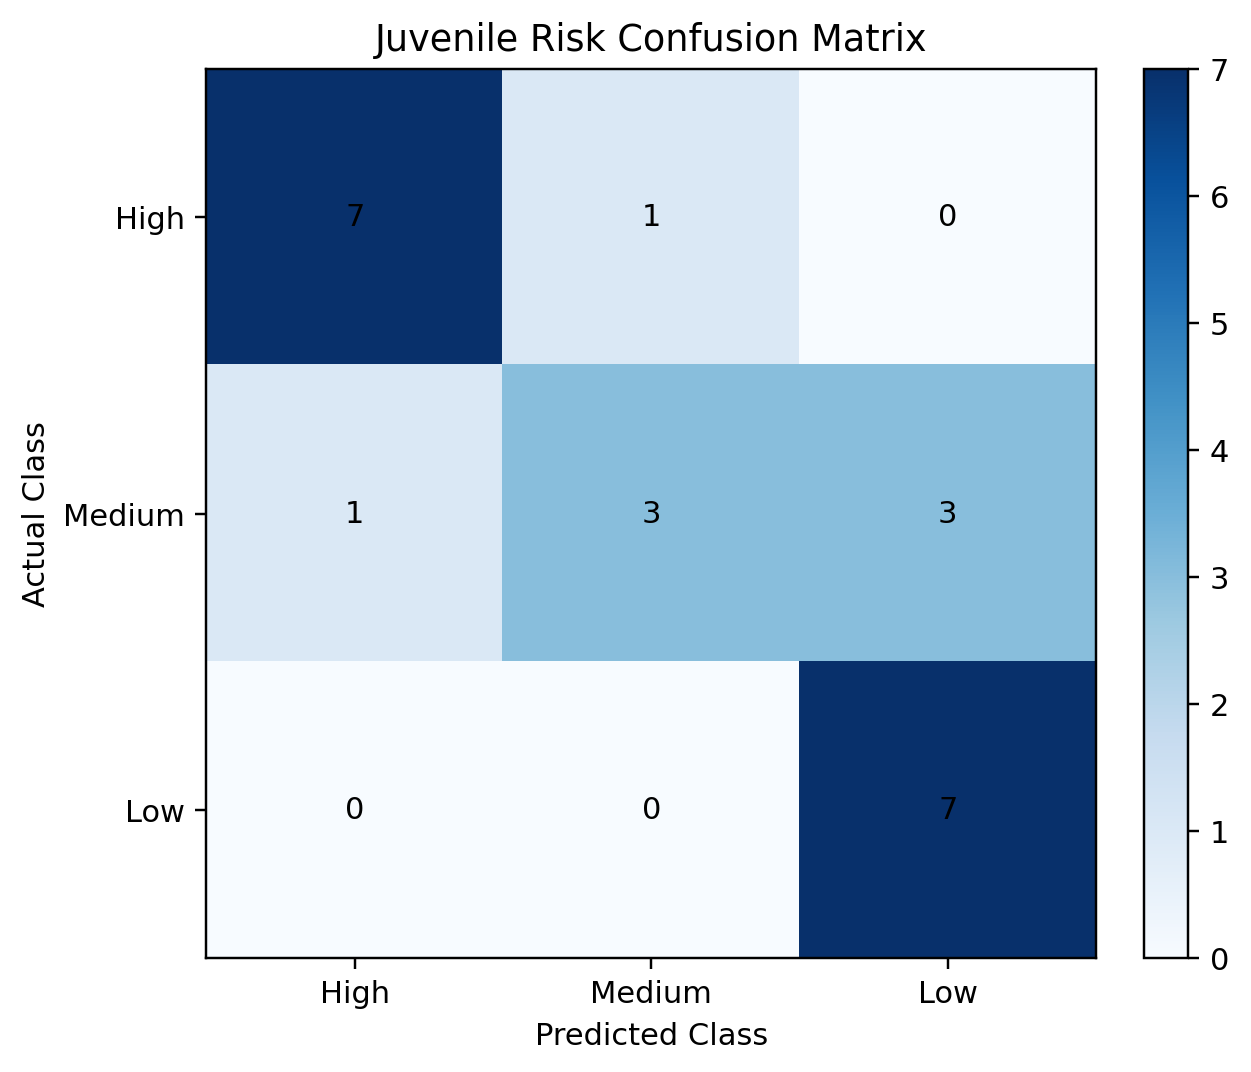
\includegraphics[width=0.66\textwidth]{reports/figures/juvenile_confusion_matrix.png}
\caption{Confusion matrix of the juvenile-risk classifier after balancing and model refinement.}
\end{figure}

\end{document}
